%!TeX spellcheck = en_GB
% Die erste (unkommentierte) Zeile im Dokument legt immer die
% Dokumentklasse fest
\documentclass{scrartcl} 

% Präambel:
% Einbinen von zusätzlichen Paketen. Falls für eine Datei keine Endung
% explizit angegeben wird, benutzt LaTeX '.tex'. Im Folgenden wird
% also die Datei 'edv_pakete.tex' eingebunden.
\input{edv_pakete}


% Verzeichnisse mit Abbildungen; kann gestrichen werden,
% falls Sie dies schon in edv_pakete.tex definiert haben:
%\graphicspath{{../report}}

\addbibresource{refs.bib} %Hinzufügen einer Literaturdatenbank aus dem angegebenen Verzeichnis

% Titel, Autor und Datum
\title{Computational Physics}
\subtitle{Exercise 2}
\date{\today}
\author{Christiane Groß, Nico Dichter}

% Jetzt startet das eigentliche Dokument
\begin{document}
	\maketitle
\section{The 2D-Ising-model}
We want to expand our solution of the Ising model in one dimension to two dimensions. For this the Hamiltoninan stays unchanged 
\begin{equation}
H(s)=-J\sum_{\langle i,j\rangle }s_is_j-h\sum_{\langle i,j\rangle }s_i
\label{eq:hamiltonianising}
\end{equation}

Here $J$ is the coupling between the nearest-neighbour-spins, $h$ is the value of the external magnetic field and the sum is over the entire lattice of size $\Lambda=N_x \cdot N_y$. In our simulations we always choose $N=N_x=N_y$.
We also know the theoretical expectation values for the  absolute value of the magnetization $|m|$ and the average energy per site $\epsilon$ when there is no external field present:
\begin{equation}
\epsilon=-J\coth(2J)\left( 1+\frac{2}{\pi}(2\tanh^2(2J)-1)K(4\sinh^2(2J)/\cosh^4(2J))\right) 
\end{equation}
\begin{equation}
|m|=\left( 1-\frac{1}{\sinh(2J)}\right)^{1/8} \text{ if } J<J_c,\quad 0 \text{ else}   
\end{equation}
 with $K(m)$ the incomplete elliptic integral of the first kind and the critical coupling $J_c=\frac{1}{2}\log(1+\sqrt{2})$. We simulate the elliptic integral with the gsl\_special-functions~\cite{gsldoc_sf}.
 
 Contrary to out simulation of the Ising model in one dimension, we do not do simple sampling here, but instead we do importance sampling. For this, we do a sweep of the entire lattice and perform an accept-reject step at each site: We propose a spin flip $s\rightarrow-s$ and accept it with probability $\min \left[1, \exp(-\Delta H/k_BT)\right]$, where $\Delta H$ is the change in energy due to the spin flip.  
%Hamiltonian, expected values for magnetization and epsilon

\section{Deliberations}
\subsection{Numerical cost of calculation}
\paragraph{Energy} Have to iterate over all lattice points: effort proportional lambda.

\paragraph{change in energy for one spin flip}
naive: calculate two Hamiltonians, subtract: scales with lambda. 
Possible: only use nearest neighbours, as shown in lecture for 1D: effort only depends ion dimension, not lattice size.

\subsection{Meaning of J} critical J: phase transition from randomly ordered to ordered.

\subsection{determining errors}

\section{simulation}
In the implementation of the simulation gsl\_matrix objects are used to save the state of the largest lattice and views on these are used to create smaller lattices (see \cite{gsldoc_mat}). For each parameter set (N,h,J) a large amount of thermalization sweeps are made and afterwards several measurements of the wanted physical variable take place with single sweeps in between. A Sweep in this case means scanning through the complete lattice and performing a Metropolis-Hastings step at each site. The thermalization steps are needed to make sure the measurements take place on configurations which resemble the given parameter set according to the boltzmann distribution. To improve the run time the function energy\_change was implemented. It calculates $\Delta S$ by only using the parts of the Hamiltonian which change when $s_{i,j}$ changes to $-s_{i,j}$, these parts consist of the energy of $s_{i,j}$ in the external magnetic field and the coppling energy with the 4 neighbours.
So in total $\Delta S$ simplifies to:
\begin{equation}
	\Delta S=2 s_{i,j}\left(\dfrac{h}{T}+\dfrac{J}{T}(s_{i+1,j}+s_{i-1,j}+s_{i,j+1}+s_{i,j-1})\right)
\end{equation}


\section{Results}

\subsection{$\langle m\rangle$ for fixed $J$ and varying $h$}
plot, description

	\begin{figure}[htbp]
		% GNUPLOT: LaTeX picture with Postscript
\begingroup
  \makeatletter
  \providecommand\color[2][]{%
    \GenericError{(gnuplot) \space\space\space\@spaces}{%
      Package color not loaded in conjunction with
      terminal option `colourtext'%
    }{See the gnuplot documentation for explanation.%
    }{Either use 'blacktext' in gnuplot or load the package
      color.sty in LaTeX.}%
    \renewcommand\color[2][]{}%
  }%
  \providecommand\includegraphics[2][]{%
    \GenericError{(gnuplot) \space\space\space\@spaces}{%
      Package graphicx or graphics not loaded%
    }{See the gnuplot documentation for explanation.%
    }{The gnuplot epslatex terminal needs graphicx.sty or graphics.sty.}%
    \renewcommand\includegraphics[2][]{}%
  }%
  \providecommand\rotatebox[2]{#2}%
  \@ifundefined{ifGPcolor}{%
    \newif\ifGPcolor
    \GPcolortrue
  }{}%
  \@ifundefined{ifGPblacktext}{%
    \newif\ifGPblacktext
    \GPblacktextfalse
  }{}%
  % define a \g@addto@macro without @ in the name:
  \let\gplgaddtomacro\g@addto@macro
  % define empty templates for all commands taking text:
  \gdef\gplbacktext{}%
  \gdef\gplfronttext{}%
  \makeatother
  \ifGPblacktext
    % no textcolor at all
    \def\colorrgb#1{}%
    \def\colorgray#1{}%
  \else
    % gray or color?
    \ifGPcolor
      \def\colorrgb#1{\color[rgb]{#1}}%
      \def\colorgray#1{\color[gray]{#1}}%
      \expandafter\def\csname LTw\endcsname{\color{white}}%
      \expandafter\def\csname LTb\endcsname{\color{black}}%
      \expandafter\def\csname LTa\endcsname{\color{black}}%
      \expandafter\def\csname LT0\endcsname{\color[rgb]{1,0,0}}%
      \expandafter\def\csname LT1\endcsname{\color[rgb]{0,1,0}}%
      \expandafter\def\csname LT2\endcsname{\color[rgb]{0,0,1}}%
      \expandafter\def\csname LT3\endcsname{\color[rgb]{1,0,1}}%
      \expandafter\def\csname LT4\endcsname{\color[rgb]{0,1,1}}%
      \expandafter\def\csname LT5\endcsname{\color[rgb]{1,1,0}}%
      \expandafter\def\csname LT6\endcsname{\color[rgb]{0,0,0}}%
      \expandafter\def\csname LT7\endcsname{\color[rgb]{1,0.3,0}}%
      \expandafter\def\csname LT8\endcsname{\color[rgb]{0.5,0.5,0.5}}%
    \else
      % gray
      \def\colorrgb#1{\color{black}}%
      \def\colorgray#1{\color[gray]{#1}}%
      \expandafter\def\csname LTw\endcsname{\color{white}}%
      \expandafter\def\csname LTb\endcsname{\color{black}}%
      \expandafter\def\csname LTa\endcsname{\color{black}}%
      \expandafter\def\csname LT0\endcsname{\color{black}}%
      \expandafter\def\csname LT1\endcsname{\color{black}}%
      \expandafter\def\csname LT2\endcsname{\color{black}}%
      \expandafter\def\csname LT3\endcsname{\color{black}}%
      \expandafter\def\csname LT4\endcsname{\color{black}}%
      \expandafter\def\csname LT5\endcsname{\color{black}}%
      \expandafter\def\csname LT6\endcsname{\color{black}}%
      \expandafter\def\csname LT7\endcsname{\color{black}}%
      \expandafter\def\csname LT8\endcsname{\color{black}}%
    \fi
  \fi
    \setlength{\unitlength}{0.0500bp}%
    \ifx\gptboxheight\undefined%
      \newlength{\gptboxheight}%
      \newlength{\gptboxwidth}%
      \newsavebox{\gptboxtext}%
    \fi%
    \setlength{\fboxrule}{0.5pt}%
    \setlength{\fboxsep}{1pt}%
\begin{picture}(8502.00,11904.00)%
    \gplgaddtomacro\gplbacktext{%
      \csname LTb\endcsname%
      \put(946,6656){\makebox(0,0)[r]{\strut{}$-1.5$}}%
      \put(946,7421){\makebox(0,0)[r]{\strut{}$-1$}}%
      \put(946,8185){\makebox(0,0)[r]{\strut{}$-0.5$}}%
      \put(946,8950){\makebox(0,0)[r]{\strut{}$0$}}%
      \put(946,9714){\makebox(0,0)[r]{\strut{}$0.5$}}%
      \put(946,10479){\makebox(0,0)[r]{\strut{}$1$}}%
      \put(946,11243){\makebox(0,0)[r]{\strut{}$1.5$}}%
      \put(1078,6436){\makebox(0,0){\strut{}$-1$}}%
      \put(2835,6436){\makebox(0,0){\strut{}$-0.5$}}%
      \put(4592,6436){\makebox(0,0){\strut{}$0$}}%
      \put(6348,6436){\makebox(0,0){\strut{}$0.5$}}%
      \put(8105,6436){\makebox(0,0){\strut{}$1$}}%
    }%
    \gplgaddtomacro\gplfronttext{%
      \csname LTb\endcsname%
      \put(176,8949){\rotatebox{-270}{\makebox(0,0){\strut{}$\langle m\rangle$}}}%
      \put(4591,6106){\makebox(0,0){\strut{}$h$}}%
      \put(4591,11573){\makebox(0,0){\strut{}$J=0.3$}}%
      \csname LTb\endcsname%
      \put(1738,11070){\makebox(0,0)[r]{\strut{}$N=$4}}%
      \csname LTb\endcsname%
      \put(1738,10850){\makebox(0,0)[r]{\strut{}$N=$8}}%
      \csname LTb\endcsname%
      \put(1738,10630){\makebox(0,0)[r]{\strut{}$N=$12}}%
      \csname LTb\endcsname%
      \put(1738,10410){\makebox(0,0)[r]{\strut{}$N=$16}}%
      \csname LTb\endcsname%
      \put(1738,10190){\makebox(0,0)[r]{\strut{}$N=$20}}%
    }%
    \gplgaddtomacro\gplbacktext{%
      \csname LTb\endcsname%
      \put(946,704){\makebox(0,0)[r]{\strut{}$-1.5$}}%
      \put(946,1469){\makebox(0,0)[r]{\strut{}$-1$}}%
      \put(946,2233){\makebox(0,0)[r]{\strut{}$-0.5$}}%
      \put(946,2998){\makebox(0,0)[r]{\strut{}$0$}}%
      \put(946,3763){\makebox(0,0)[r]{\strut{}$0.5$}}%
      \put(946,4527){\makebox(0,0)[r]{\strut{}$1$}}%
      \put(946,5292){\makebox(0,0)[r]{\strut{}$1.5$}}%
      \put(1078,484){\makebox(0,0){\strut{}$-1$}}%
      \put(2835,484){\makebox(0,0){\strut{}$-0.5$}}%
      \put(4592,484){\makebox(0,0){\strut{}$0$}}%
      \put(6348,484){\makebox(0,0){\strut{}$0.5$}}%
      \put(8105,484){\makebox(0,0){\strut{}$1$}}%
    }%
    \gplgaddtomacro\gplfronttext{%
      \csname LTb\endcsname%
      \put(176,2998){\rotatebox{-270}{\makebox(0,0){\strut{}$\langle m\rangle$}}}%
      \put(4591,154){\makebox(0,0){\strut{}$h$}}%
      \put(4591,5622){\makebox(0,0){\strut{}$J=0.8$}}%
      \csname LTb\endcsname%
      \put(1738,5119){\makebox(0,0)[r]{\strut{}$N=$4}}%
      \csname LTb\endcsname%
      \put(1738,4899){\makebox(0,0)[r]{\strut{}$N=$8}}%
      \csname LTb\endcsname%
      \put(1738,4679){\makebox(0,0)[r]{\strut{}$N=$12}}%
      \csname LTb\endcsname%
      \put(1738,4459){\makebox(0,0)[r]{\strut{}$N=$16}}%
      \csname LTb\endcsname%
      \put(1738,4239){\makebox(0,0)[r]{\strut{}$N=$20}}%
    }%
    \gplbacktext
    \put(0,0){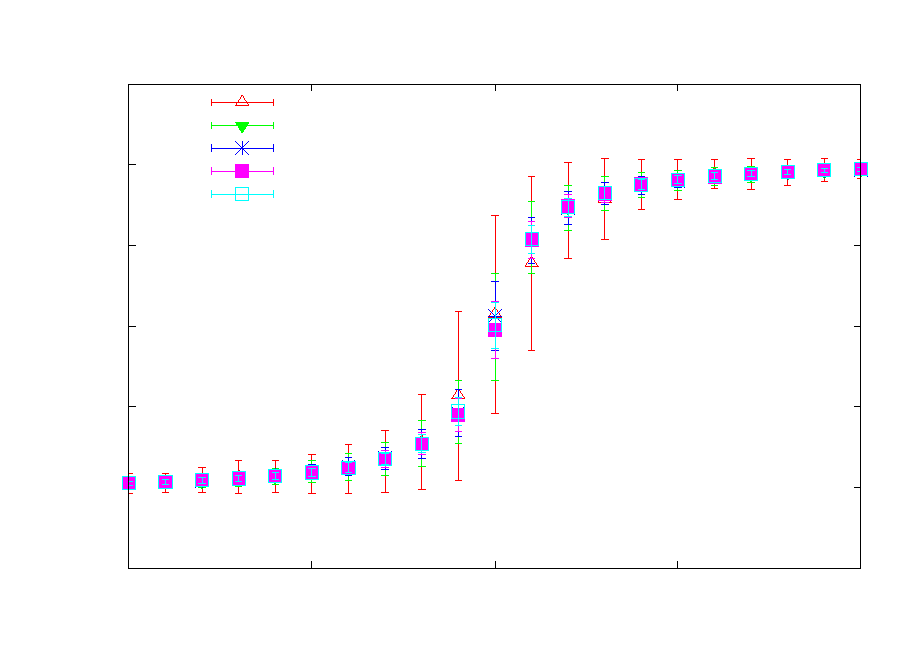
\includegraphics{magnetizationfixJ}}%
    \gplfronttext
  \end{picture}%
\endgroup

		\caption{Magnetization for two differerent values of fixed $J$}
		\label{fig:magfixJ}
	\end{figure}

\subsection{$\langle \epsilon\rangle$ for fixed $h=0$ and varying $J$}
plot, description, comparison literature
	\begin{figure}[htbp]
		% GNUPLOT: LaTeX picture with Postscript
\begingroup
  \makeatletter
  \providecommand\color[2][]{%
    \GenericError{(gnuplot) \space\space\space\@spaces}{%
      Package color not loaded in conjunction with
      terminal option `colourtext'%
    }{See the gnuplot documentation for explanation.%
    }{Either use 'blacktext' in gnuplot or load the package
      color.sty in LaTeX.}%
    \renewcommand\color[2][]{}%
  }%
  \providecommand\includegraphics[2][]{%
    \GenericError{(gnuplot) \space\space\space\@spaces}{%
      Package graphicx or graphics not loaded%
    }{See the gnuplot documentation for explanation.%
    }{The gnuplot epslatex terminal needs graphicx.sty or graphics.sty.}%
    \renewcommand\includegraphics[2][]{}%
  }%
  \providecommand\rotatebox[2]{#2}%
  \@ifundefined{ifGPcolor}{%
    \newif\ifGPcolor
    \GPcolortrue
  }{}%
  \@ifundefined{ifGPblacktext}{%
    \newif\ifGPblacktext
    \GPblacktextfalse
  }{}%
  % define a \g@addto@macro without @ in the name:
  \let\gplgaddtomacro\g@addto@macro
  % define empty templates for all commands taking text:
  \gdef\gplbacktext{}%
  \gdef\gplfronttext{}%
  \makeatother
  \ifGPblacktext
    % no textcolor at all
    \def\colorrgb#1{}%
    \def\colorgray#1{}%
  \else
    % gray or color?
    \ifGPcolor
      \def\colorrgb#1{\color[rgb]{#1}}%
      \def\colorgray#1{\color[gray]{#1}}%
      \expandafter\def\csname LTw\endcsname{\color{white}}%
      \expandafter\def\csname LTb\endcsname{\color{black}}%
      \expandafter\def\csname LTa\endcsname{\color{black}}%
      \expandafter\def\csname LT0\endcsname{\color[rgb]{1,0,0}}%
      \expandafter\def\csname LT1\endcsname{\color[rgb]{0,1,0}}%
      \expandafter\def\csname LT2\endcsname{\color[rgb]{0,0,1}}%
      \expandafter\def\csname LT3\endcsname{\color[rgb]{1,0,1}}%
      \expandafter\def\csname LT4\endcsname{\color[rgb]{0,1,1}}%
      \expandafter\def\csname LT5\endcsname{\color[rgb]{1,1,0}}%
      \expandafter\def\csname LT6\endcsname{\color[rgb]{0,0,0}}%
      \expandafter\def\csname LT7\endcsname{\color[rgb]{1,0.3,0}}%
      \expandafter\def\csname LT8\endcsname{\color[rgb]{0.5,0.5,0.5}}%
    \else
      % gray
      \def\colorrgb#1{\color{black}}%
      \def\colorgray#1{\color[gray]{#1}}%
      \expandafter\def\csname LTw\endcsname{\color{white}}%
      \expandafter\def\csname LTb\endcsname{\color{black}}%
      \expandafter\def\csname LTa\endcsname{\color{black}}%
      \expandafter\def\csname LT0\endcsname{\color{black}}%
      \expandafter\def\csname LT1\endcsname{\color{black}}%
      \expandafter\def\csname LT2\endcsname{\color{black}}%
      \expandafter\def\csname LT3\endcsname{\color{black}}%
      \expandafter\def\csname LT4\endcsname{\color{black}}%
      \expandafter\def\csname LT5\endcsname{\color{black}}%
      \expandafter\def\csname LT6\endcsname{\color{black}}%
      \expandafter\def\csname LT7\endcsname{\color{black}}%
      \expandafter\def\csname LT8\endcsname{\color{black}}%
    \fi
  \fi
    \setlength{\unitlength}{0.0500bp}%
    \ifx\gptboxheight\undefined%
      \newlength{\gptboxheight}%
      \newlength{\gptboxwidth}%
      \newsavebox{\gptboxtext}%
    \fi%
    \setlength{\fboxrule}{0.5pt}%
    \setlength{\fboxsep}{1pt}%
\begin{picture}(8502.00,6008.00)%
    \gplgaddtomacro\gplbacktext{%
      \csname LTb\endcsname%
      \put(946,704){\makebox(0,0)[r]{\strut{}$-4$}}%
      \put(946,1334){\makebox(0,0)[r]{\strut{}$-3.5$}}%
      \put(946,1964){\makebox(0,0)[r]{\strut{}$-3$}}%
      \put(946,2594){\makebox(0,0)[r]{\strut{}$-2.5$}}%
      \put(946,3224){\makebox(0,0)[r]{\strut{}$-2$}}%
      \put(946,3853){\makebox(0,0)[r]{\strut{}$-1.5$}}%
      \put(946,4483){\makebox(0,0)[r]{\strut{}$-1$}}%
      \put(946,5113){\makebox(0,0)[r]{\strut{}$-0.5$}}%
      \put(946,5743){\makebox(0,0)[r]{\strut{}$0$}}%
      \put(1680,484){\makebox(0,0){\strut{}$0.4$}}%
      \put(2483,484){\makebox(0,0){\strut{}$0.6$}}%
      \put(3286,484){\makebox(0,0){\strut{}$0.8$}}%
      \put(4090,484){\makebox(0,0){\strut{}$1$}}%
      \put(4893,484){\makebox(0,0){\strut{}$1.2$}}%
      \put(5696,484){\makebox(0,0){\strut{}$1.4$}}%
      \put(6499,484){\makebox(0,0){\strut{}$1.6$}}%
      \put(7302,484){\makebox(0,0){\strut{}$1.8$}}%
      \put(8105,484){\makebox(0,0){\strut{}$2$}}%
    }%
    \gplgaddtomacro\gplfronttext{%
      \csname LTb\endcsname%
      \put(176,3223){\rotatebox{-270}{\makebox(0,0){\strut{}$\langle\epsilon\rangle$}}}%
      \put(4591,154){\makebox(0,0){\strut{}$J$}}%
      \put(4591,5633){\makebox(0,0){\strut{}}}%
      \csname LTb\endcsname%
      \put(7118,5570){\makebox(0,0)[r]{\strut{}theory}}%
      \csname LTb\endcsname%
      \put(7118,5350){\makebox(0,0)[r]{\strut{}$N=$4}}%
      \csname LTb\endcsname%
      \put(7118,5130){\makebox(0,0)[r]{\strut{}$N=$8}}%
      \csname LTb\endcsname%
      \put(7118,4910){\makebox(0,0)[r]{\strut{}$N=$12}}%
      \csname LTb\endcsname%
      \put(7118,4690){\makebox(0,0)[r]{\strut{}$N=$16}}%
      \csname LTb\endcsname%
      \put(7118,4470){\makebox(0,0)[r]{\strut{}$N=$20}}%
    }%
    \gplbacktext
    \put(0,0){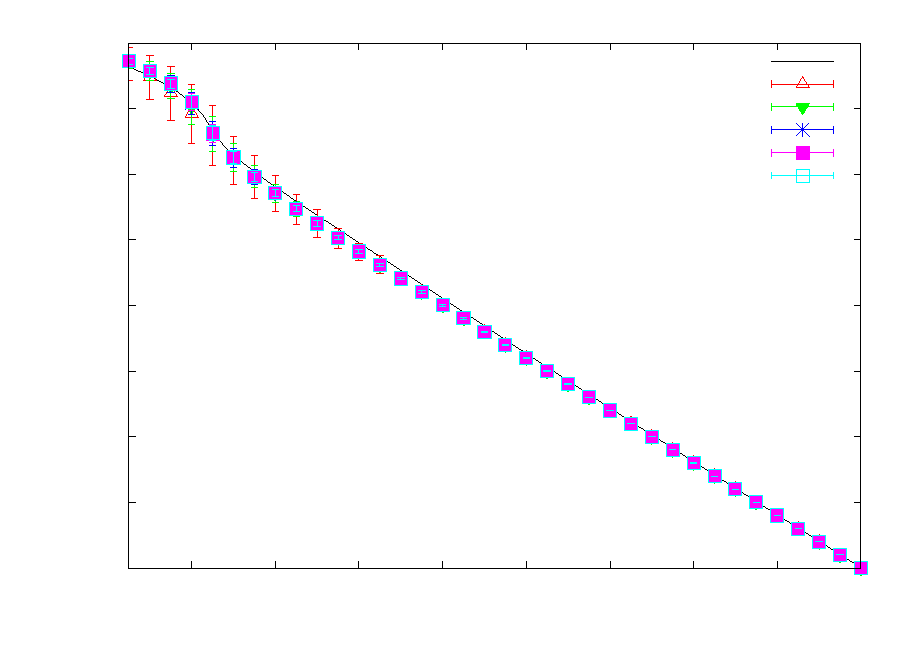
\includegraphics{avenergy}}%
    \gplfronttext
  \end{picture}%
\endgroup

		\caption{Average energy per site for $h=0$}
		\label{fig:energy}
	\end{figure}

\subsection{$\langle |m|\rangle$ for fixed $h$ and varying $J$}
plot, description, comparison literature

	\begin{figure}[htbp]
		\input{absmagnetization}
		\caption{Modulus of magnetization for $h=0$}
		\label{fig:absmag}
	\end{figure}
see sharp drop, phase transition
\paragraph{$\langle |m|\rangle$ vs. $\langle m\rangle$}
For $h=0$: everything cancels out, m=0 everywhere because simulation randomly flops between positive and negative behaviour, even at ordered phase due to finite length.
Use absolute value of m so it can't cancel out.

\paragraph{thermodynamical limit}



\newpage	
\listoffigures
\printbibliography
\end{document}